% ============================================================
%  appendices/S3_metric_reporting.tex
% ============================================================

\section{Asymmetric Fairness-Metric Reporting Across the Corpus}
\label{app:S3}

Figure~\ref{fig:metric_reporting} summarises the reporting rates for
standard performance metrics and fairness-specific metrics across the
78~included studies, illustrating the marked asymmetry between the
two classes.

% ─── Metric-reporting figure ──────────────────────────────
\begin{figure}[!ht]
  \centering
  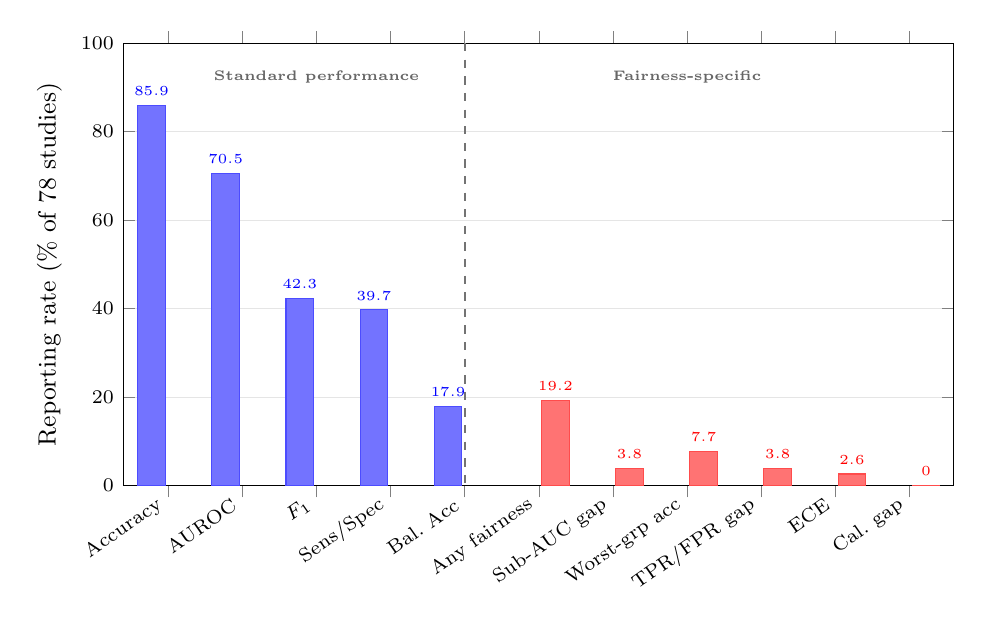
\begin{tikzpicture}
    \begin{axis}[
        width=\linewidth, height=7.2cm,
        ybar, bar width=10pt,
        ymin=0, ymax=100,
        ylabel={Reporting rate (\% of 78 studies)},
        ylabel style={font=\small},
        tick label style={font=\scriptsize},
        xtick={Acc,AUROC,F1,Sens/Spec,BalAcc,
               AnyFair,SubAUC,WGAcc,TPR/FPR,ECE,CalGap},
        symbolic x coords={Acc,AUROC,F1,Sens/Spec,BalAcc,
                           AnyFair,SubAUC,WGAcc,TPR/FPR,ECE,CalGap},
        xticklabels={Accuracy, AUROC, $F_1$, Sens/Spec, Bal.\ Acc,
                     Any fairness, Sub-AUC gap, Worst-grp acc,
                     TPR/FPR gap, ECE, Cal.\ gap},
        x tick label style={rotate=35, anchor=east, align=right,
                            font=\scriptsize},
        nodes near coords, nodes near coords style={font=\tiny},
        enlarge x limits=0.06,
        major grid style={draw=black!10},
        ymajorgrids=true,
      ]
      % Standard performance metrics (blue)
      \addplot+[fill=blue!55, draw=blue!70]
        coordinates {(Acc,85.9) (AUROC,70.5) (F1,42.3)
                     (Sens/Spec,39.7) (BalAcc,17.9)};
      % Fairness-specific metrics (red)
      \addplot+[fill=red!55, draw=red!70]
        coordinates {(AnyFair,19.2) (SubAUC,3.8) (WGAcc,7.7)
                     (TPR/FPR,3.8) (ECE,2.6) (CalGap,0.0)};
      \draw[dashed, black!55, thick]
        ({axis cs:BalAcc,0}|-{rel axis cs:0,1}) -- ({axis cs:BalAcc,0});
      \node[anchor=north, font=\tiny, text=black!60]
        at (axis cs:F1,96)    {\textbf{Standard performance}};
      \node[anchor=north, font=\tiny, text=black!60]
        at (axis cs:WGAcc,96)  {\textbf{Fairness-specific}};
    \end{axis}
  \end{tikzpicture}
  \caption{\textbf{Asymmetric reporting of performance versus fairness
           metrics across the 78 included histopathology
           studies.}  Reporting rates are from systematic audit of
           the full analytical corpus.  Aggregate performance metrics
           (accuracy 85.9\%, AUROC 70.5\%, $F_1$ 42.3\%) are
           near-universally reported, whereas any fairness-specific
           metric appears in only 19.2\% of studies ($n=15$).
           Worst-group accuracy/AUC --- the minimum fairness guarantee
           demanded by recent regulatory guidance --- is reported in
           only 7.7\% ($n=6$ studies); Expected Calibration
           Error~(ECE) in 2.6\% ($n=2$); and the
           \emph{subgroup calibration gap} in none.  The dashed
           vertical rule separates standard performance metrics (left,
           blue) from fairness metrics (right, red).  This reporting
           asymmetry implies that the empirical base for evaluating
           debiasing is drawn from a small, selection-biased subset
           and is the principal reason that evidence grades in
           Figure~\ref{fig:mitigation_grid} and
           Table~\ref{tab:mitigation_summary} rest on a limited
           number of studies.}
  \label{fig:metric_reporting}
\end{figure}
